\Exercise[number={14}]
A variable \(x\) in \(\mathbb{R}^2\) is emitted by two possible sources,
\(w_1\) and \(w_2\), with equal a-priori probabilities \(Pr(w_1)=Pr(w_2)\).
We want to design a Bayes classifier that assigns the correct class to
each observed \(x\). The \(p(x|w_i)\) both have a Gaussian distribution,
multivariate with means \(\mu_1\) and \(\mu_2\) and covariance
matrices \(\Sigma_1\) and \(\Sigma_2\).\\
a. Find an expression for the discriminant function \(z(x)\) in the
general case \(\mu_1\neq\mu_2\) and \(\Sigma_1\neq\Sigma_2\).\\
b. If \(\mu_1=(-a,0)\), \(\mu_2=(a,0)\), \(\Sigma_1=diag(1,2)\) and
\(\Sigma_2=diag(1,1)\) where \(a\) is a parameter, determine (for \(a>0\),
\(a<0\), and \(a=0\)) the locus of the points for which \(z(x)=0\).\\
c. Display graphically (under hypothesis b.) as accurately as possible
the contour of the decision regions.

\Answer[number={14}]
a. The discriminant function \(z(x)\) can be computed as follow:
\begin{align*}
    z(x)
    &=\log{\frac{p(x|w_1)}{p(x|w_2)}}+\cancel{\log{\frac{Pr(w_1)}{Pr(w_2)}}}
    =\log{p(x|w_1)}-\log{p(x|w_2)}\\
    &=-\frac{1}{2}\log{|\Sigma_1|}-\frac{1}{2}(x-\mu_1)^T\Sigma_1^{-1}(x-\mu_1)+\frac{1}{2}\log{|\Sigma_2|}+\frac{1}{2}(x-\mu_2)^T\Sigma_2^{-1}(x-\mu_2)\\
    &=\frac{1}{2}\log{\frac{|\Sigma_2|}{|\Sigma_1|}}-\frac{1}{2}(x-\mu_1)^T\Sigma_1^{-1}(x-\mu_1)+\frac{1}{2}(x-\mu_2)^T\Sigma_2^{-1}(x-\mu_2)
\end{align*}
b. Let's substitute the parameters' values into \(z(x)\):
\begin{align*}
    z(x)
    &=\frac{1}{2}\log{\frac{1}{2}}-\frac{1}{2}
    \begin{bmatrix}
        x_1+a && x_2
    \end{bmatrix}
    \begin{bmatrix}
        1 && 0 \\ 0 && \frac{1}{2}
    \end{bmatrix}
    \begin{bmatrix}
        x_1+a \\ x_2
    \end{bmatrix}
    +\frac{1}{2}
    \begin{bmatrix}
        x_1-a && x_2
    \end{bmatrix}
    \begin{bmatrix}
        1 && 0 \\ 0 && 1
    \end{bmatrix}
    \begin{bmatrix}
        x_1-a \\ x_2
    \end{bmatrix}\\
    &=-\frac{1}{2}\log{2}-\frac{1}{2}
    \begin{bmatrix}
        x_1+a && \frac{1}{2}x_2
    \end{bmatrix}
    \begin{bmatrix}
        x_1+a && x_2
    \end{bmatrix}
    +\frac{1}{2}
    \begin{bmatrix}
        x_1-a && x_2
    \end{bmatrix}
    \begin{bmatrix}
        x_1-a \\ x_2
    \end{bmatrix}\\
    &=-\frac{1}{2}\log{2}-\frac{1}{2}\bigl[(x_1+a)^2+\frac{1}{2}x_2^2\bigr]+\frac{1}{2}\bigl[(x_1-a)^2+x_2^2\bigr]\\
    &=-\frac{1}{2}\log{2}-\cancel{\frac{1}{2}x_1^2}-\cancel{\frac{1}{2}a^2}-ax_1-\frac{1}{4}x_2^2+\cancel{\frac{1}{2}x_1^2}+\cancel{\frac{1}{2}a^2}-ax_1+\frac{1}{2}x_2^2\\
    &=-\frac{1}{2}\log{2}-2ax_1+\frac{1}{4}x_2^2
\end{align*}
The decision boundary is obtained for \(z(x)=0\):
\begin{align*}
    z(x)=0
    \Longleftrightarrow
    -\frac{1}{2}\log{2}-2ax_1+\frac{1}{4}x_2^2=0
    \Rightarrow
    x_2^2=4(\frac{1}{2}\log{2}+2ax_1)
    \Rightarrow
    x_2=\pm\sqrt{4(\frac{1}{2}\log{2}+2ax_1)}
\end{align*}
Notice that for \(a=0\) the means of the two Gaussian distributions are
coincident, thus there is no decision boundary. While \(a>0\) the plot
on the left side is obtained, the one on the right side is instead
drawn for \(a<0\).
\begin{figure}[H]
    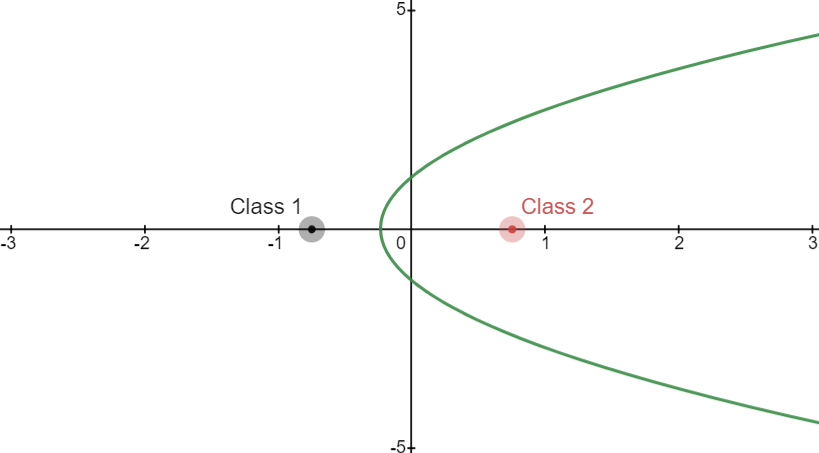
\includegraphics[scale=0.45]{C_14_1}
    \hspace{1cm}
    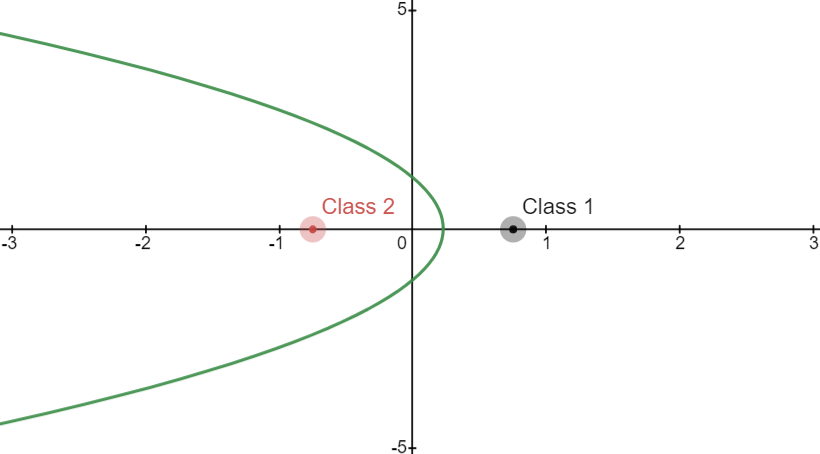
\includegraphics[scale=0.45]{C_14_2}
    \centering
\end{figure}